\begin{frame}{(Continuous) Integration of scientific software}
    \framesubtitle{Hands on: setup a Gitlab runner I (install Gitlab runner)}
    Using instructions from \href{https://docs.gitlab.com/runner/install/linux-repository.html}{Gitlab documentation} for Ubuntu:
    \begin{enumerate}
        \item \mint[fontsize=\footnotesize]{bash}+?> curl -L \ +
              \mint[fontsize=\footnotesize]{bash}+"https://packages.gitlab.com/install/repositories/runner/gitlab-runner/script.deb.sh" \ +
              \mint[fontsize=\footnotesize]{bash}+  | sudo bash+
        \item \mint[fontsize=\footnotesize]{bash}+?> sudo apt-get install gitlab-runner+
    \end{enumerate}
    Check the status of the runner:
    \begin{itemize}
        \item \mint{bash}+?> sudo systemctl status gitlab-runner.service+
    \end{itemize}
    The output should indicate that it is active:
    \begin{figure}
        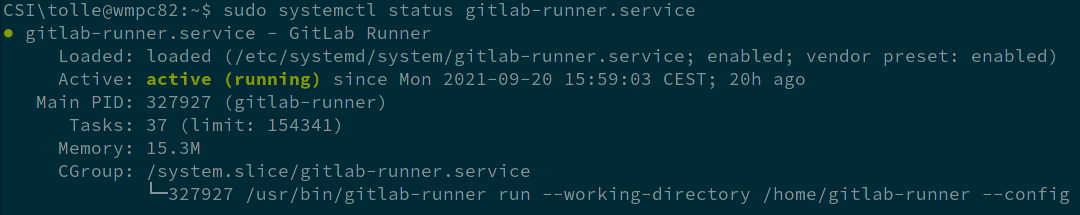
\includegraphics[width=0.75\textwidth]{figures/gitlab-runner-active.png}
    \end{figure}
\end{frame}


\begin{frame}{(Continuous) Integration of scientific software}
    \framesubtitle{Hands on: setup a Gitlab runner II (register Gitlab runner)}
    Follow GitLab documentation on \href{https://docs.gitlab.com/runner/register/index.html}{how to register a runner}:
    \begin{itemize}
        \item Obtain a token for project-specific runner: go to your fork of the \emph{minimal-cse-example} on gitlab.com and then to \textbf{Settings > CI/CD} and expand the \textbf{Runners} sections.
        \item There you find a section \textbf{Specific runners} and aforementioned token.
    \end{itemize}
    Register your runner (instructions for Linux):
    \begin{itemize}
        \item \mint{bash}+?> sudo gitlab-runner register+
    \end{itemize}
    You need to provide some information regarding your runner, e.g. your project's token. See next slide.
\end{frame}


\begin{frame}{(Continuous) Integration of scientific software}
    \framesubtitle{Hands on: setup a Gitlab runner III (register Gitlab runner)}
    \begin{table}
        \begin{tabularx}{\textwidth}{l|X}
            \textbf{Option}              & \textbf{Value} \\
            \hline
            GitLab instance URL & https://gitlab.com/ \\
            Token               & Obtained from the project on GitLab, see previous slide \\
            Runner description  & describe the machine used as runner, useful to distinguish multiple runners \\
            Tags                & leave empty, not required here. Useful for advanced pipelines \\
            Runner executor     & docker (see \href{https://docs.gitlab.com/runner/executors/}{here} for comparison of executors.)\\
            Default image       & Because we chose docker as executor: name of the default Docker image
        \end{tabularx}
    \end{table}
    \begin{columns}[t]
        \begin{column}{0.5\textwidth}
        You should now see your runner under \newline \emph{Available specific runners}:
        \end{column}

        \begin{column}{0.5\textwidth}
            \begin{figure}[T!]
                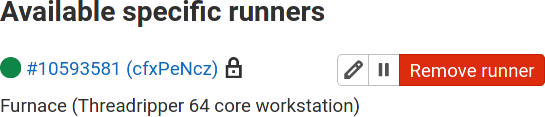
\includegraphics[width=0.9\textwidth]{figures/runner-registered.png}
            \end{figure}
        \end{column}
    \end{columns}
\end{frame}


%\begin{frame}{(Continuous) Integration of scientific software}
%    \framesubtitle{Hands on: setup a Gitlab runner IV (configure Gitlab runner)}
%    You can further adapt your runner configuration by editing
%    \href{https://docs.gitlab.com/runner/configuration/advanced-configuration.html}{/etc/gitlab-runner}
%\end{frame}
